% Options for packages loaded elsewhere
\PassOptionsToPackage{unicode}{hyperref}
\PassOptionsToPackage{hyphens}{url}
%
\documentclass[
]{book}
\usepackage{amsmath,amssymb}
\usepackage{lmodern}
\usepackage{iftex}
\ifPDFTeX
  \usepackage[T1]{fontenc}
  \usepackage[utf8]{inputenc}
  \usepackage{textcomp} % provide euro and other symbols
\else % if luatex or xetex
  \usepackage{unicode-math}
  \defaultfontfeatures{Scale=MatchLowercase}
  \defaultfontfeatures[\rmfamily]{Ligatures=TeX,Scale=1}
\fi
% Use upquote if available, for straight quotes in verbatim environments
\IfFileExists{upquote.sty}{\usepackage{upquote}}{}
\IfFileExists{microtype.sty}{% use microtype if available
  \usepackage[]{microtype}
  \UseMicrotypeSet[protrusion]{basicmath} % disable protrusion for tt fonts
}{}
\makeatletter
\@ifundefined{KOMAClassName}{% if non-KOMA class
  \IfFileExists{parskip.sty}{%
    \usepackage{parskip}
  }{% else
    \setlength{\parindent}{0pt}
    \setlength{\parskip}{6pt plus 2pt minus 1pt}}
}{% if KOMA class
  \KOMAoptions{parskip=half}}
\makeatother
\usepackage{xcolor}
\IfFileExists{xurl.sty}{\usepackage{xurl}}{} % add URL line breaks if available
\IfFileExists{bookmark.sty}{\usepackage{bookmark}}{\usepackage{hyperref}}
\hypersetup{
  pdftitle={Annalyse de données},
  pdfauthor={Abdoul Oudouss Diakite, Othmane ETTADLAOUI},
  hidelinks,
  pdfcreator={LaTeX via pandoc}}
\urlstyle{same} % disable monospaced font for URLs
\usepackage{color}
\usepackage{fancyvrb}
\newcommand{\VerbBar}{|}
\newcommand{\VERB}{\Verb[commandchars=\\\{\}]}
\DefineVerbatimEnvironment{Highlighting}{Verbatim}{commandchars=\\\{\}}
% Add ',fontsize=\small' for more characters per line
\usepackage{framed}
\definecolor{shadecolor}{RGB}{248,248,248}
\newenvironment{Shaded}{\begin{snugshade}}{\end{snugshade}}
\newcommand{\AlertTok}[1]{\textcolor[rgb]{0.94,0.16,0.16}{#1}}
\newcommand{\AnnotationTok}[1]{\textcolor[rgb]{0.56,0.35,0.01}{\textbf{\textit{#1}}}}
\newcommand{\AttributeTok}[1]{\textcolor[rgb]{0.77,0.63,0.00}{#1}}
\newcommand{\BaseNTok}[1]{\textcolor[rgb]{0.00,0.00,0.81}{#1}}
\newcommand{\BuiltInTok}[1]{#1}
\newcommand{\CharTok}[1]{\textcolor[rgb]{0.31,0.60,0.02}{#1}}
\newcommand{\CommentTok}[1]{\textcolor[rgb]{0.56,0.35,0.01}{\textit{#1}}}
\newcommand{\CommentVarTok}[1]{\textcolor[rgb]{0.56,0.35,0.01}{\textbf{\textit{#1}}}}
\newcommand{\ConstantTok}[1]{\textcolor[rgb]{0.00,0.00,0.00}{#1}}
\newcommand{\ControlFlowTok}[1]{\textcolor[rgb]{0.13,0.29,0.53}{\textbf{#1}}}
\newcommand{\DataTypeTok}[1]{\textcolor[rgb]{0.13,0.29,0.53}{#1}}
\newcommand{\DecValTok}[1]{\textcolor[rgb]{0.00,0.00,0.81}{#1}}
\newcommand{\DocumentationTok}[1]{\textcolor[rgb]{0.56,0.35,0.01}{\textbf{\textit{#1}}}}
\newcommand{\ErrorTok}[1]{\textcolor[rgb]{0.64,0.00,0.00}{\textbf{#1}}}
\newcommand{\ExtensionTok}[1]{#1}
\newcommand{\FloatTok}[1]{\textcolor[rgb]{0.00,0.00,0.81}{#1}}
\newcommand{\FunctionTok}[1]{\textcolor[rgb]{0.00,0.00,0.00}{#1}}
\newcommand{\ImportTok}[1]{#1}
\newcommand{\InformationTok}[1]{\textcolor[rgb]{0.56,0.35,0.01}{\textbf{\textit{#1}}}}
\newcommand{\KeywordTok}[1]{\textcolor[rgb]{0.13,0.29,0.53}{\textbf{#1}}}
\newcommand{\NormalTok}[1]{#1}
\newcommand{\OperatorTok}[1]{\textcolor[rgb]{0.81,0.36,0.00}{\textbf{#1}}}
\newcommand{\OtherTok}[1]{\textcolor[rgb]{0.56,0.35,0.01}{#1}}
\newcommand{\PreprocessorTok}[1]{\textcolor[rgb]{0.56,0.35,0.01}{\textit{#1}}}
\newcommand{\RegionMarkerTok}[1]{#1}
\newcommand{\SpecialCharTok}[1]{\textcolor[rgb]{0.00,0.00,0.00}{#1}}
\newcommand{\SpecialStringTok}[1]{\textcolor[rgb]{0.31,0.60,0.02}{#1}}
\newcommand{\StringTok}[1]{\textcolor[rgb]{0.31,0.60,0.02}{#1}}
\newcommand{\VariableTok}[1]{\textcolor[rgb]{0.00,0.00,0.00}{#1}}
\newcommand{\VerbatimStringTok}[1]{\textcolor[rgb]{0.31,0.60,0.02}{#1}}
\newcommand{\WarningTok}[1]{\textcolor[rgb]{0.56,0.35,0.01}{\textbf{\textit{#1}}}}
\usepackage{longtable,booktabs,array}
\usepackage{calc} % for calculating minipage widths
% Correct order of tables after \paragraph or \subparagraph
\usepackage{etoolbox}
\makeatletter
\patchcmd\longtable{\par}{\if@noskipsec\mbox{}\fi\par}{}{}
\makeatother
% Allow footnotes in longtable head/foot
\IfFileExists{footnotehyper.sty}{\usepackage{footnotehyper}}{\usepackage{footnote}}
\makesavenoteenv{longtable}
\usepackage{graphicx}
\makeatletter
\def\maxwidth{\ifdim\Gin@nat@width>\linewidth\linewidth\else\Gin@nat@width\fi}
\def\maxheight{\ifdim\Gin@nat@height>\textheight\textheight\else\Gin@nat@height\fi}
\makeatother
% Scale images if necessary, so that they will not overflow the page
% margins by default, and it is still possible to overwrite the defaults
% using explicit options in \includegraphics[width, height, ...]{}
\setkeys{Gin}{width=\maxwidth,height=\maxheight,keepaspectratio}
% Set default figure placement to htbp
\makeatletter
\def\fps@figure{htbp}
\makeatother
\setlength{\emergencystretch}{3em} % prevent overfull lines
\providecommand{\tightlist}{%
  \setlength{\itemsep}{0pt}\setlength{\parskip}{0pt}}
\setcounter{secnumdepth}{5}
\usepackage{booktabs}
\ifLuaTeX
  \usepackage{selnolig}  % disable illegal ligatures
\fi
\usepackage[]{natbib}
\bibliographystyle{plainnat}

\title{Annalyse de données}
\author{Abdoul Oudouss Diakite, Othmane ETTADLAOUI}
\date{01 June, 2022}

\begin{document}
\maketitle

{
\setcounter{tocdepth}{1}
\tableofcontents
}
\hypertarget{introduction}{%
\chapter*{Introduction}\label{introduction}}
\addcontentsline{toc}{chapter}{Introduction}

Ce projet d'analyse de donnés consiste à l'explication de différentes manières le nombre de crime aux Etats-Unis. Pour se faire, nous disposons d'un jeu de disponible sur GitHub que nous appellerons \texttt{Comminities}(\href{https://github.com/AODiakite/Data-Analysis/blob/main/data/Communities.csv}{\emph{Télécharger}}) dorénavant.\\

\begin{tabular}{l|l|l|l|r|r|r|r|r|r|r|r|r|r|r|r|r|r|r|r|r|r|r|r|r|r|r|r|r|r|l|r|r|r|r|r|r|r|r|r|r|r|r|r|r|r|r|r|r|r|r|r|r|r|r|r|r|r|r|r|r|r|r|r|r|r|r|r|r|r|r|r|r|r|r|r|r|r|r|r|r|r|r|r|r|r|r|r|r|r|r|r|r|r|r|r|r|r|r|r|r|r|r|l|l|l|l|l|l|l|l|l|l|l|l|l|l|l|l|l|r|r|r|l|l|l|l|r|l|r|r|l|l|l|l|l|l|l|l|l|l|l|l|l|l|l|l}
\hline
communityname & State & countyCode & communityCode & fold & pop & perHoush & pctBlack & pctWhite & pctAsian & pctHisp & pct12.21 & pct12.29 & pct16.24 & pct65up & persUrban & pctUrban & medIncome & pctWwage & pctWfarm & pctWdiv & pctWsocsec & pctPubAsst & pctRetire & medFamIncome & perCapInc & whitePerCap & blackPerCap & NAperCap & asianPerCap & otherPerCap & hispPerCap & persPoverty & pctPoverty & pctLowEdu & pctNotHSgrad & pctCollGrad & pctUnemploy & pctEmploy & pctEmployMfg & pctEmployProfServ & pctOccupManu & pctOccupMgmt & pctMaleDivorc & pctMaleNevMar & pctFemDivorc & pctAllDivorc & persPerFam & pct2Par & pctKids2Par & pctKids.4w2Par & pct12.17w2Par & pctWorkMom.6 & pctWorkMom.18 & kidsBornNevrMarr & pctKidsBornNevrMarr & numForeignBorn & pctFgnImmig.3 & pctFgnImmig.5 & pctFgnImmig.8 & pctFgnImmig.10 & pctImmig.3 & pctImmig.5 & pctImmig.8 & pctImmig.10 & pctSpeakOnlyEng & pctNotSpeakEng & pctLargHousFam & pctLargHous & persPerOccupHous & persPerOwnOccup & persPerRenterOccup & pctPersOwnOccup & pctPopDenseHous & pctSmallHousUnits & medNumBedrm & houseVacant & pctHousOccup & pctHousOwnerOccup & pctVacantBoarded & pctVacant6up & medYrHousBuilt & pctHousWOphone & pctHousWOplumb & ownHousLowQ & ownHousMed & ownHousUperQ & ownHousQrange & rentLowQ & rentMed & rentUpperQ & rentQrange & medGrossRent & medRentpctHousInc & medOwnCostpct & medOwnCostPctWO & persEmergShelt & persHomeless & pctForeignBorn & pctBornStateResid & pctSameHouse.5 & pctSameCounty.5 & pctSameState.5 & numPolice & policePerPop & policeField & policeFieldPerPop & policeCalls & policCallPerPop & policCallPerOffic & policePerPop2 & racialMatch & pctPolicWhite & pctPolicBlack & pctPolicHisp & pctPolicAsian & pctPolicMinority & officDrugUnits & numDiffDrugsSeiz & policAveOT & landArea & popDensity & pctUsePubTrans & policCarsAvail & policOperBudget & pctPolicPatrol & gangUnit & pctOfficDrugUnit & policBudgetPerPop & murders & murdPerPop & rapes & rapesPerPop & robberies & robbbPerPop & assaults & assaultPerPop & burglaries & burglPerPop & larcenies & larcPerPop & autoTheft & autoTheftPerPop & arsons & arsonsPerPop & violentPerPop & nonViolPerPop\\
\hline
BerkeleyHeightstownship & NJ & 39 & 5320 & 1 & 11980 & 3.10 & 1.37 & 91.78 & 6.50 & 1.88 & 12.47 & 21.44 & 10.93 & 11.33 & 11980 & 100 & 75122 & 89.24 & 1.55 & 70.20 & 23.62 & 1.03 & 18.39 & 79584 & 29711 & 30233 & 13600 & 5725 & 27101 & 5115 & 22838 & 227 & 1.96 & 5.81 & 9.90 & 48.18 & 2.70 & 64.55 & 14.65 & 28.82 & 5.49 & 50.73 & 3.67 & 26.38 & 5.22 & 4.47 & 3.22 & 91.43 & 90.17 & 95.78 & 95.81 & 44.56 & 58.88 & 31 & 0.36 & 1277 & 8.69 & 13.00 & 20.99 & 30.93 & 0.93 & 1.39 & 2.24 & 3.30 & 85.68 & 1.37 & 4.81 & 4.17 & 2.99 & 3.00 & 2.84 & 91.46 & 0.39 & 11.06 & 3 & 64 & 98.37 & 91.01 & 3.12 & 37.50 & 1959 & 0.00 & 0.28 & 215900 & 262600 & 326900 & 111000 & 685 & 1001 & 1001 & 316 & 1001 & 23.8 & 21.1 & 14.0 & 11 & 0 & 10.66 & 53.72 & 65.29 & 78.09 & 89.14 & ? & ? & ? & ? & ? & ? & ? & ? & ? & ? & ? & ? & ? & ? & ? & ? & ? & 6.5 & 1845.9 & 9.63 & ? & ? & ? & ? & 0 & ? & 0 & 0.0 & 0 & 0 & 1 & 8.2 & 4 & 32.81 & 14 & 114.85 & 138 & 1132.08 & 16 & 131.26 & 2 & 16.41 & 41.02 & 1394.59\\
\hline
Marpletownship & PA & 45 & 47616 & 1 & 23123 & 2.82 & 0.80 & 95.57 & 3.44 & 0.85 & 11.01 & 21.30 & 10.48 & 17.18 & 23123 & 100 & 47917 & 78.99 & 1.11 & 64.11 & 35.50 & 2.75 & 22.85 & 55323 & 20148 & 20191 & 18137 & 0 & 20074 & 5250 & 12222 & 885 & 3.98 & 5.61 & 13.72 & 29.89 & 2.43 & 61.96 & 12.26 & 29.28 & 6.39 & 37.64 & 4.23 & 27.99 & 6.45 & 5.42 & 3.11 & 86.91 & 85.33 & 96.82 & 86.46 & 51.14 & 62.43 & 43 & 0.24 & 1920 & 5.21 & 8.65 & 13.33 & 22.50 & 0.43 & 0.72 & 1.11 & 1.87 & 87.79 & 1.81 & 4.25 & 3.34 & 2.70 & 2.83 & 1.96 & 89.03 & 1.01 & 23.60 & 3 & 240 & 97.15 & 84.88 & 0.00 & 18.33 & 1958 & 0.31 & 0.14 & 136300 & 164200 & 199900 & 63600 & 467 & 560 & 672 & 205 & 627 & 27.6 & 20.7 & 12.5 & 0 & 0 & 8.30 & 77.17 & 71.27 & 90.22 & 96.12 & ? & ? & ? & ? & ? & ? & ? & ? & ? & ? & ? & ? & ? & ? & ? & ? & ? & 10.6 & 2186.7 & 3.84 & ? & ? & ? & ? & 0 & ? & 0 & 0.0 & 1 & 4.25 & 5 & 21.26 & 24 & 102.05 & 57 & 242.37 & 376 & 1598.78 & 26 & 110.55 & 1 & 4.25 & 127.56 & 1955.95\\
\hline
Tigardcity & OR & ? & ? & 1 & 29344 & 2.43 & 0.74 & 94.33 & 3.43 & 2.35 & 11.36 & 25.88 & 11.01 & 10.28 & 29344 & 100 & 35669 & 82.00 & 1.15 & 55.73 & 22.25 & 2.94 & 14.56 & 42112 & 16946 & 17103 & 16644 & 21606 & 15528 & 5954 & 8405 & 1389 & 4.75 & 2.80 & 9.09 & 30.13 & 4.01 & 69.80 & 15.95 & 21.52 & 8.79 & 32.48 & 10.10 & 25.78 & 14.76 & 12.55 & 2.95 & 78.54 & 78.85 & 92.37 & 75.72 & 66.08 & 74.19 & 164 & 0.88 & 1468 & 16.42 & 23.98 & 32.08 & 35.63 & 0.82 & 1.20 & 1.61 & 1.78 & 93.11 & 1.14 & 2.97 & 2.05 & 2.42 & 2.69 & 2.06 & 64.18 & 2.03 & 47.46 & 3 & 544 & 95.68 & 57.79 & 0.92 & 7.54 & 1976 & 1.55 & 0.12 & 74700 & 90400 & 112000 & 37300 & 370 & 428 & 520 & 150 & 484 & 24.1 & 21.7 & 11.6 & 16 & 0 & 5.00 & 44.77 & 36.60 & 61.26 & 82.85 & ? & ? & ? & ? & ? & ? & ? & ? & ? & ? & ? & ? & ? & ? & ? & ? & ? & 10.6 & 2780.9 & 4.37 & ? & ? & ? & ? & 0 & ? & 3 & 8.3 & 6 & 16.6 & 56 & 154.95 & 14 & 38.74 & 274 & 758.14 & 1797 & 4972.19 & 136 & 376.3 & 22 & 60.87 & 218.59 & 6167.51\\
\hline
Gloversvillecity & NY & 35 & 29443 & 1 & 16656 & 2.40 & 1.70 & 97.35 & 0.50 & 0.70 & 12.55 & 25.20 & 12.19 & 17.57 & 0 & 0 & 20580 & 68.15 & 0.24 & 38.95 & 39.48 & 11.71 & 18.33 & 26501 & 10810 & 10909 & 9984 & 4941 & 3541 & 2451 & 4391 & 2831 & 17.23 & 11.05 & 33.68 & 10.81 & 9.86 & 54.74 & 31.22 & 27.43 & 26.76 & 22.71 & 10.98 & 28.15 & 14.47 & 12.91 & 2.98 & 64.02 & 62.36 & 65.38 & 67.43 & 59.59 & 70.27 & 561 & 3.84 & 339 & 13.86 & 13.86 & 15.34 & 15.34 & 0.28 & 0.28 & 0.31 & 0.31 & 94.98 & 0.56 & 3.93 & 2.56 & 2.37 & 2.51 & 2.20 & 58.18 & 1.21 & 45.66 & 3 & 669 & 91.19 & 54.89 & 2.54 & 57.85 & 1939 & 7.00 & 0.87 & 36400 & 49600 & 66500 & 30100 & 195 & 250 & 309 & 114 & 333 & 28.7 & 20.6 & 14.5 & 0 & 0 & 2.04 & 88.71 & 56.70 & 90.17 & 96.24 & ? & ? & ? & ? & ? & ? & ? & ? & ? & ? & ? & ? & ? & ? & ? & ? & ? & 5.2 & 3217.7 & 3.31 & ? & ? & ? & ? & 0 & ? & 0 & 0.0 & 10 & 57.86 & 10 & 57.86 & 33 & 190.93 & 225 & 1301.78 & 716 & 4142.56 & 47 & 271.93 & ? & ? & 306.64 & ?\\
\hline
Bemidjicity & MN & 7 & 5068 & 1 & 11245 & 2.76 & 0.53 & 89.16 & 1.17 & 0.52 & 24.46 & 40.53 & 28.69 & 12.65 & 0 & 0 & 17390 & 69.33 & 0.55 & 42.82 & 32.16 & 11.21 & 14.43 & 24018 & 8483 & 9009 & 887 & 4425 & 3352 & 3000 & 1328 & 2855 & 29.99 & 12.15 & 23.06 & 25.28 & 9.08 & 52.44 & 6.89 & 36.54 & 10.94 & 27.80 & 7.51 & 50.66 & 11.64 & 9.73 & 2.98 & 58.59 & 55.20 & 66.51 & 79.17 & 61.22 & 68.94 & 402 & 4.70 & 196 & 46.94 & 56.12 & 67.86 & 69.90 & 0.82 & 0.98 & 1.18 & 1.22 & 94.64 & 0.39 & 5.23 & 3.11 & 2.35 & 2.55 & 2.12 & 58.13 & 2.94 & 55.64 & 2 & 333 & 92.45 & 53.57 & 3.90 & 42.64 & 1958 & 7.45 & 0.82 & 30600 & 43200 & 59500 & 28900 & 202 & 283 & 362 & 160 & 332 & 32.2 & 23.2 & 12.9 & 2 & 0 & 1.74 & 73.75 & 42.22 & 60.34 & 89.02 & ? & ? & ? & ? & ? & ? & ? & ? & ? & ? & ? & ? & ? & ? & ? & ? & ? & 11.5 & 974.2 & 0.38 & ? & ? & ? & ? & 0 & ? & 0 & 0.0 & ? & ? & 4 & 32.04 & 14 & 112.14 & 91 & 728.93 & 1060 & 8490.87 & 91 & 728.93 & 5 & 40.05 & ? & 9988.79\\
\hline
\end{tabular}

\hypertarget{description-du-jeu-de-donnuxe9es}{%
\section*{Description du jeu de données}\label{description-du-jeu-de-donnuxe9es}}
\addcontentsline{toc}{section}{Description du jeu de données}

Le jeu de données dispose de 147 variables pour 2215 observations. Les valeurs manquantes sont représentées par \texttt{"?"}.\\
De nombreuses variables sont incluses afin que les algorithmes qui sélectionnent ou apprennent les poids des attributs puissent être testés. Cependant, les attributs clairement non liés n'ont pas été inclus; les attributs ont été sélectionnés s'il y avait un lien plausible avec la criminalité (N = 125), plus les variables de criminalité qui sont des variables dépendantes potentielles. Les variables incluses dans l'ensemble de données impliquent la communauté, telles que le pourcentage de la population considérée comme urbaine et le revenu familial médian, et impliquent l'application de la loi, telles que le nombre d'agents de police par habitant et le pourcentage d'agents affectés aux unités de lutte contre la drogue. Les attributs de crime (N = 18) qui pourraient être prédits sont les 8 crimes considérés comme des «crimes indexés» par le FBI (Meurtres, viols, vols qualifiés, \ldots. ), versions par habitant (en fait pour 100 000 habitants) de chacun, et crimes violents par habitant et crimes non violents par habitant).\\
Pour faciliter la tâche aux lecteurs de se projet, nous avons créés un fichier csv nommé \texttt{Description.csv}(\href{https://github.com/AODiakite/Data-Analysis/blob/main/data/Description.csv}{\emph{Télécharger}}) qui contient les noms des variables dans la colonne \texttt{feature} et leur descriptions dans la colonne \texttt{Description}

\begin{tabular}{l|l}
\hline
feature & Description\\
\hline
communityname & Community name - not predictive - for information only (string)\\
\hline
state & US state (by 2 letter postal abbreviation)(nominal)\\
\hline
countyCode & numeric code for county - not predictive, and many missing values (numeric)\\
\hline
communityCode & numeric code for community - not predictive and many missing values (numeric)\\
\hline
fold & fold number for non-random 10 fold cross validation, potentially useful for debugging, paired tests - not predictive (numeric - integer)\\
\hline
population & population for community\\
\hline
\end{tabular}

\hypertarget{source-des-donnuxe9es}{%
\section{Source des données}\label{source-des-donnuxe9es}}

\emph{UCI Machine Learning}\footnote{\url{https://archive.ics.uci.edu/ml/datasets/Communities+and+Crime+Unnormalized\#}}\strut \\
@ref1
@ref2
@ref3
@ref4

\hypertarget{linearModel}{%
\chapter{Régression linéaire}\label{linearModel}}

\hypertarget{introduction-1}{%
\section{Introduction}\label{introduction-1}}

La régression lineaire est une méthode statistique qui permet de trouver une relation lineaire entre des variables quantitives, une à expliquer et d'autres explicatives. C'est en fait un ajustement affine de la forme :

\begin{equation}
y_i = \beta_0 + \beta_1x_{i1} + \beta_2x_{i2} +\dots+\beta_px_{ip}+\epsilon_{i}\;\; 
\end{equation}

\[i\in\{1,2,3\dots,n\}\]

\begin{itemize}
\tightlist
\item
  \(y_i\) représentent la \(i\)ème valeur de la variable dépendantes \(y\).
\item
  \(x_{ij}\) représente la mesure de la \(i\)ème observation de la variable explicative \(X_j\)
\item
  les \(\beta_j\) sont les paramètres inconnus du modèle à estimer
\item
  \(\epsilon_i\) représente le bruit associé à la \(i\)ème observation\\
\end{itemize}

L'équation précédente peut être écrite sous une forme matricielle de cette manière :\\

\begin{equation}
y = X\beta +\epsilon
\end{equation}

avec :\\

\begin{equation}
y = \begin{pmatrix}y_1\\y_2\\\vdots\\y_n \end{pmatrix} \;\; 
X = \begin{pmatrix}
   1 & x_{11} & x_{12} & \dots &x_{1p}\\
   1 & x_{21} & x_{22} & \dots &x_{2p}\\
   \vdots &\vdots&\vdots & &\vdots\\
   1 & x_{n1} & x_{n2} & \dots &x_{np}
   \end{pmatrix} \;\;
\beta = \begin{pmatrix}\beta_0\\
   \beta_1\\
   \vdots\\
   \beta_n \end{pmatrix} \;\;
\epsilon = \begin{pmatrix}
   \epsilon_1\\
   \epsilon_2\\
   \vdots\\
   \epsilon_n \end{pmatrix} \;\;
\end{equation}

\hfill\break

Commençons par importer le jeu de données que nous nommerons \(dfcom\):\\

\begin{Shaded}
\begin{Highlighting}[]
\NormalTok{Communities }\OtherTok{=} \FunctionTok{read.csv}\NormalTok{(}\StringTok{"data/Communities.csv"}\NormalTok{,}\AttributeTok{row.names =} \DecValTok{1}\NormalTok{)}
\end{Highlighting}
\end{Shaded}

\begin{tabular}{l|l|l|l|r|r|r|r|r|r|r|r|r|r|r}
\hline
communityname & State & countyCode & communityCode & fold & pop & perHoush & pctBlack & pctWhite & pctAsian & pctHisp & pct12.21 & pct12.29 & pct16.24 & pct65up\\
\hline
BerkeleyHeightstownship & NJ & 39 & 5320 & 1 & 11980 & 3.10 & 1.37 & 91.78 & 6.50 & 1.88 & 12.47 & 21.44 & 10.93 & 11.33\\
\hline
Marpletownship & PA & 45 & 47616 & 1 & 23123 & 2.82 & 0.80 & 95.57 & 3.44 & 0.85 & 11.01 & 21.30 & 10.48 & 17.18\\
\hline
Tigardcity & OR & ? & ? & 1 & 29344 & 2.43 & 0.74 & 94.33 & 3.43 & 2.35 & 11.36 & 25.88 & 11.01 & 10.28\\
\hline
Gloversvillecity & NY & 35 & 29443 & 1 & 16656 & 2.40 & 1.70 & 97.35 & 0.50 & 0.70 & 12.55 & 25.20 & 12.19 & 17.57\\
\hline
Bemidjicity & MN & 7 & 5068 & 1 & 11245 & 2.76 & 0.53 & 89.16 & 1.17 & 0.52 & 24.46 & 40.53 & 28.69 & 12.65\\
\hline
Springfieldcity & MO & ? & ? & 1 & 140494 & 2.45 & 2.51 & 95.65 & 0.90 & 0.95 & 18.09 & 32.89 & 20.04 & 13.26\\
\hline
Norwoodtown & MA & 21 & 50250 & 1 & 28700 & 2.60 & 1.60 & 96.57 & 1.47 & 1.10 & 11.17 & 27.41 & 12.76 & 14.42\\
\hline
Andersoncity & IN & ? & ? & 1 & 59459 & 2.45 & 14.20 & 84.87 & 0.40 & 0.63 & 15.31 & 27.93 & 14.78 & 14.60\\
\hline
Fargocity & ND & 17 & 25700 & 1 & 74111 & 2.46 & 0.35 & 97.11 & 1.25 & 0.73 & 16.64 & 35.16 & 20.33 & 8.58\\
\hline
Wacocity & TX & ? & ? & 1 & 103590 & 2.62 & 23.14 & 67.60 & 0.92 & 16.35 & 19.88 & 34.55 & 21.62 & 13.12\\
\hline
\end{tabular}

\hypertarget{application-de-la-ruxe9gression-linuxe9aire-simple}{%
\section{Application de la régression linéaire simple}\label{application-de-la-ruxe9gression-linuxe9aire-simple}}

\hypertarget{corruxe9lation}{%
\subsection*{Corrélation}\label{corruxe9lation}}
\addcontentsline{toc}{subsection}{Corrélation}

Comme nous l'avons mentionner dans l'introduction, le but de se projet est d'expliquer de différentes manières les meurtes aux USA. Par conséquent, on peut choisir comme variable dépendante, les crimes(\texttt{murders}) et chercher les variables explicatives. Dans le cas de le régression linéaire simple il doit exister une corrélation assez importante entre la variable \(y\)(\texttt{muders}) et \(X\) que nous recherchons actuellement. Donc commençons par filtrer les fortes corrélation avec la variable \(y\) dans notre jeu de données.\\

\begin{Shaded}
\begin{Highlighting}[]
\CommentTok{\# Correlation matrix}
\NormalTok{corCom }\OtherTok{=}\NormalTok{ correlation}\SpecialCharTok{::}\FunctionTok{correlation}\NormalTok{(Communities)}
\CommentTok{\# Filtered correlation, bound =0.8}
\NormalTok{corCom[(corCom}\SpecialCharTok{$}\NormalTok{r}\SpecialCharTok{\textgreater{}}\FloatTok{0.8}\NormalTok{) }\SpecialCharTok{\&}\NormalTok{ corCom}\SpecialCharTok{$}\NormalTok{Parameter2}\SpecialCharTok{==}\StringTok{\textquotesingle{}murders\textquotesingle{}}\NormalTok{,]}
\end{Highlighting}
\end{Shaded}

\begin{verbatim}
## # Correlation Matrix (pearson-method)
## 
## Parameter1       | Parameter2 |    r |       95% CI | t(2213) |         p
## -------------------------------------------------------------------------
## pop              |    murders | 0.96 | [0.96, 0.96] |  159.80 | < .001***
## persUrban        |    murders | 0.96 | [0.95, 0.96] |  156.13 | < .001***
## persPoverty      |    murders | 0.98 | [0.97, 0.98] |  211.42 | < .001***
## kidsBornNevrMarr |    murders | 0.98 | [0.98, 0.98] |  221.27 | < .001***
## numForeignBorn   |    murders | 0.89 | [0.88, 0.90] |   92.94 | < .001***
## houseVacant      |    murders | 0.90 | [0.89, 0.90] |   95.29 | < .001***
## persEmergShelt   |    murders | 0.89 | [0.88, 0.90] |   93.14 | < .001***
## persHomeless     |    murders | 0.85 | [0.84, 0.86] |   76.49 | < .001***
## 
## p-value adjustment method: Holm (1979)
## Observations: 2215
\end{verbatim}

\hypertarget{nuage-de-points}{%
\subsection*{Nuage de points}\label{nuage-de-points}}
\addcontentsline{toc}{subsection}{Nuage de points}

Le tableau précédent indique les variables fortement corrélées avec notre \(output\) \texttt{murders}. Prenons l'exemple de la variable \texttt{persPoverty} qui représente le nombre de personnes sous le seuil de pauvreté.\\

\begin{Shaded}
\begin{Highlighting}[]
\FunctionTok{library}\NormalTok{(ggplot2)}
\NormalTok{fig }\OtherTok{=} \FunctionTok{ggplot}\NormalTok{(}\AttributeTok{data =}\NormalTok{ Communities,}\FunctionTok{aes}\NormalTok{(}\AttributeTok{x=}\NormalTok{persPoverty,}\AttributeTok{y=}\NormalTok{murders))}\SpecialCharTok{+}
  \FunctionTok{geom\_point}\NormalTok{()}
\NormalTok{fig}
\end{Highlighting}
\end{Shaded}

\begin{center}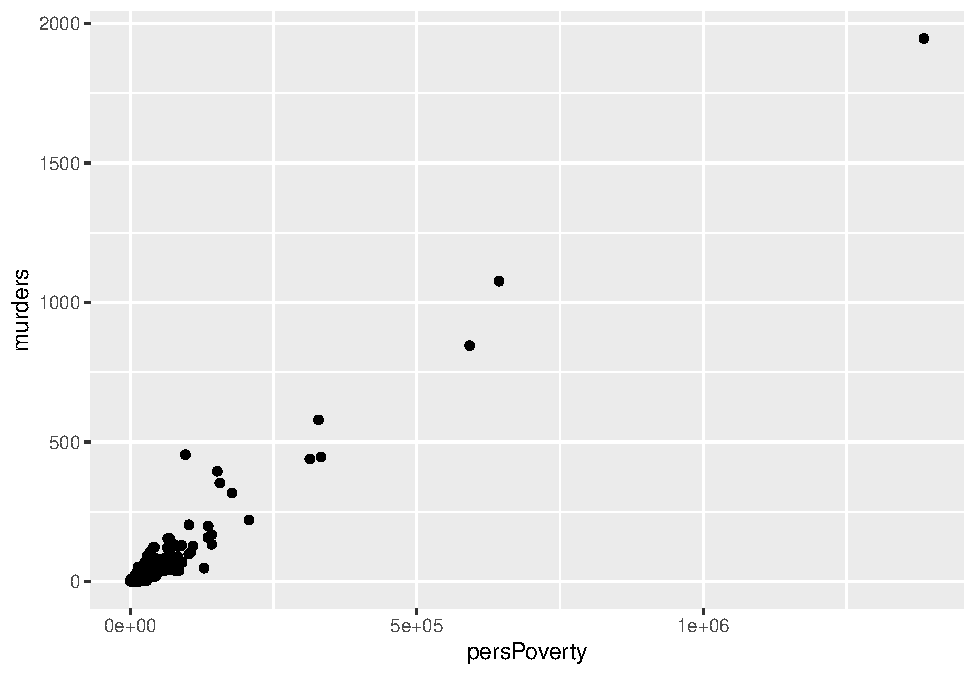
\includegraphics{_main_files/figure-latex/unnamed-chunk-8-1} \end{center}

\hypertarget{entrauxeenement-de-moduxe8le-droite-de-ruxe9gression}{%
\subsection*{Entraînement de modèle \& Droite de régression}\label{entrauxeenement-de-moduxe8le-droite-de-ruxe9gression}}
\addcontentsline{toc}{subsection}{Entraînement de modèle \& Droite de régression}

La figure précédente laisse parraître qu'il pourrait effectivement exister une relation linéaire entre \texttt{murders} et \texttt{persPoverty}. Appliquons la fonction \texttt{lm()} pour voir ce qu'il en est vraiment ! Pour faire une analyse des résidus pltard, nous n'entrainerons que \(75\%\) du jeu de données et le reste servira à la prédiction.\\

\begin{Shaded}
\begin{Highlighting}[]
\FunctionTok{library}\NormalTok{(dplyr)}
\CommentTok{\# Train\_Test\_Splite}
\FunctionTok{set.seed}\NormalTok{(}\DecValTok{1345}\NormalTok{)}
\CommentTok{\# Pourcentage de donnees correspondant a 25\%}
\NormalTok{per }\OtherTok{=} \FunctionTok{dim}\NormalTok{(Communities)[}\DecValTok{1}\NormalTok{]}\SpecialCharTok{\%/\%}\DecValTok{4}
\NormalTok{echantillon }\OtherTok{\textless{}{-}} \FunctionTok{sample}\NormalTok{(}\DecValTok{1}\SpecialCharTok{:}\FunctionTok{dim}\NormalTok{(Communities)[}\DecValTok{1}\NormalTok{]) }\SpecialCharTok{\%\textgreater{}\%}\NormalTok{ .[}\DecValTok{1}\SpecialCharTok{:}\NormalTok{per]}
\NormalTok{lmDataTrain }\OtherTok{=}\NormalTok{ Communities[}\SpecialCharTok{{-}}\NormalTok{echantillon,}\FunctionTok{c}\NormalTok{(}\StringTok{"murders"}\NormalTok{,}\StringTok{"persPoverty"}\NormalTok{)]}
\NormalTok{lmDataTest }\OtherTok{=}\NormalTok{ Communities[echantillon,}\FunctionTok{c}\NormalTok{(}\StringTok{"murders"}\NormalTok{,}\StringTok{"persPoverty"}\NormalTok{)]}
\end{Highlighting}
\end{Shaded}

\begin{Shaded}
\begin{Highlighting}[]
\CommentTok{\#Model Training}
\NormalTok{lmSimple }\OtherTok{\textless{}{-}} \FunctionTok{lm}\NormalTok{(murders}\SpecialCharTok{\textasciitilde{}}\NormalTok{persPoverty,}\AttributeTok{data =}\NormalTok{ lmDataTrain)}
\FunctionTok{summary}\NormalTok{(lmSimple)}
\end{Highlighting}
\end{Shaded}

\begin{verbatim}
## 
## Call:
## lm(formula = murders ~ persPoverty, data = lmDataTrain)
## 
## Residuals:
##     Min      1Q  Median      3Q     Max 
## -136.43   -1.13    1.32    2.52  317.80 
## 
## Coefficients:
##               Estimate Std. Error t value Pr(>|t|)    
## (Intercept) -3.271e+00  3.340e-01  -9.796   <2e-16 ***
## persPoverty  1.449e-03  7.447e-06 194.519   <2e-16 ***
## ---
## Signif. codes:  0 '***' 0.001 '**' 0.01 '*' 0.05 '.' 0.1 ' ' 1
## 
## Residual standard error: 13.4 on 1660 degrees of freedom
## Multiple R-squared:  0.958,  Adjusted R-squared:  0.9579 
## F-statistic: 3.784e+04 on 1 and 1660 DF,  p-value: < 2.2e-16
\end{verbatim}

La sortie de la fonction \texttt{summary()} indique des \(p-values\) très inférieures à \(5\%\), donc on rejette l'hypothèse de nullité des \(\beta\). On peut aussi constater que le coefficient de détermination \(R^2\) vaut \(0.958\) ce qui signifie que notre modèle a un score de \(95.8\%\). Ce dernier reflète une bonne qualité du modèle.\\

\begin{Shaded}
\begin{Highlighting}[]
\NormalTok{ggstatsplot}\SpecialCharTok{::}\FunctionTok{ggscatterstats}\NormalTok{(}
  \AttributeTok{data =}\NormalTok{ lmDataTrain, }
  \AttributeTok{x =}\NormalTok{ persPoverty, }
  \AttributeTok{y =}\NormalTok{ murders,}
  \AttributeTok{xlab  =} \StringTok{"le nombre de personnes sous le seuil de pauvreté"}\NormalTok{,}
  \AttributeTok{ylab  =} \StringTok{"le nombre de meurtres"}\NormalTok{,}
  \AttributeTok{title =} \StringTok{"Droite de régression"}\NormalTok{,}
  \AttributeTok{messages =} \ConstantTok{FALSE}
\NormalTok{)}
\end{Highlighting}
\end{Shaded}

\begin{verbatim}
## Registered S3 method overwritten by 'ggside':
##   method from   
##   +.gg   ggplot2
\end{verbatim}

\begin{verbatim}
## `stat_bin()` using `bins = 30`. Pick better value with `binwidth`.
## `stat_bin()` using `bins = 30`. Pick better value with `binwidth`.
\end{verbatim}

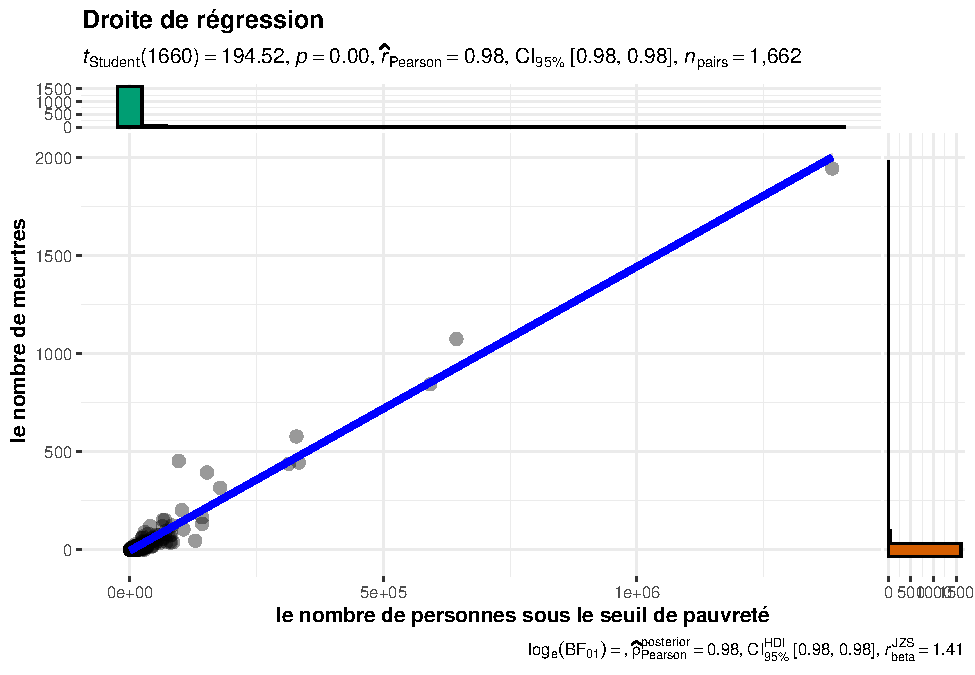
\includegraphics{_main_files/figure-latex/unnamed-chunk-11-1.pdf}

\hypertarget{pruxe9diction}{%
\subsection*{Prédiction}\label{pruxe9diction}}
\addcontentsline{toc}{subsection}{Prédiction}

A présent, nous pouvons utiliser notre échantillon non entrainé de données pour prédire à partir de notre model, quel aurait était le nombre de meurtres pour chauque \(x_i\).\\

\begin{Shaded}
\begin{Highlighting}[]
\NormalTok{X\_test}\OtherTok{=}\FunctionTok{as.data.frame}\NormalTok{(lmDataTest[[}\StringTok{"persPoverty"}\NormalTok{]])}
\FunctionTok{colnames}\NormalTok{(X\_test)}\OtherTok{=}\StringTok{"persPoverty"}
\NormalTok{y\_predict }\OtherTok{=} \FunctionTok{predict}\NormalTok{(}\AttributeTok{object =}\NormalTok{ lmSimple,X\_test)}
\end{Highlighting}
\end{Shaded}

\hypertarget{graphes-des-ruxe9sidus}{%
\subsection*{Graphes des résidus}\label{graphes-des-ruxe9sidus}}
\addcontentsline{toc}{subsection}{Graphes des résidus}

On peut représenter le graphe des \(\hat y\) prédits et des \(y\). Pour un modèle parfait, le nuage de point doit être sur la première bissectrice.\\

\begin{Shaded}
\begin{Highlighting}[]
\FunctionTok{ggplot}\NormalTok{(}\AttributeTok{data =}\NormalTok{lmDataTest) }\SpecialCharTok{+}
  \FunctionTok{geom\_point}\NormalTok{(}\FunctionTok{aes}\NormalTok{(persPoverty,murders),}\AttributeTok{color =} \StringTok{\textquotesingle{}darkgreen\textquotesingle{}}\NormalTok{,}
             \AttributeTok{size =}\DecValTok{2}\NormalTok{,}\AttributeTok{shape=}\DecValTok{22}\NormalTok{,}\AttributeTok{fill =}\StringTok{"darkgreen"}\NormalTok{) }\SpecialCharTok{+}
  \FunctionTok{geom\_point}\NormalTok{(}\FunctionTok{aes}\NormalTok{(}\AttributeTok{x =}\NormalTok{ persPoverty, }\AttributeTok{y =}\NormalTok{y\_predict), }\AttributeTok{color =}\StringTok{\textquotesingle{}blue\textquotesingle{}}\NormalTok{) }\SpecialCharTok{+}
  \FunctionTok{geom\_segment}\NormalTok{(}\FunctionTok{aes}\NormalTok{(}\AttributeTok{x =}\NormalTok{persPoverty , }
                   \AttributeTok{y =}\NormalTok{ murders, }\AttributeTok{xend =}\NormalTok{ persPoverty, }\AttributeTok{yend =}\NormalTok{ y\_predict),}
               \AttributeTok{color =} \StringTok{\textquotesingle{}red\textquotesingle{}}\NormalTok{)}
\end{Highlighting}
\end{Shaded}

\begin{figure}

{\centering 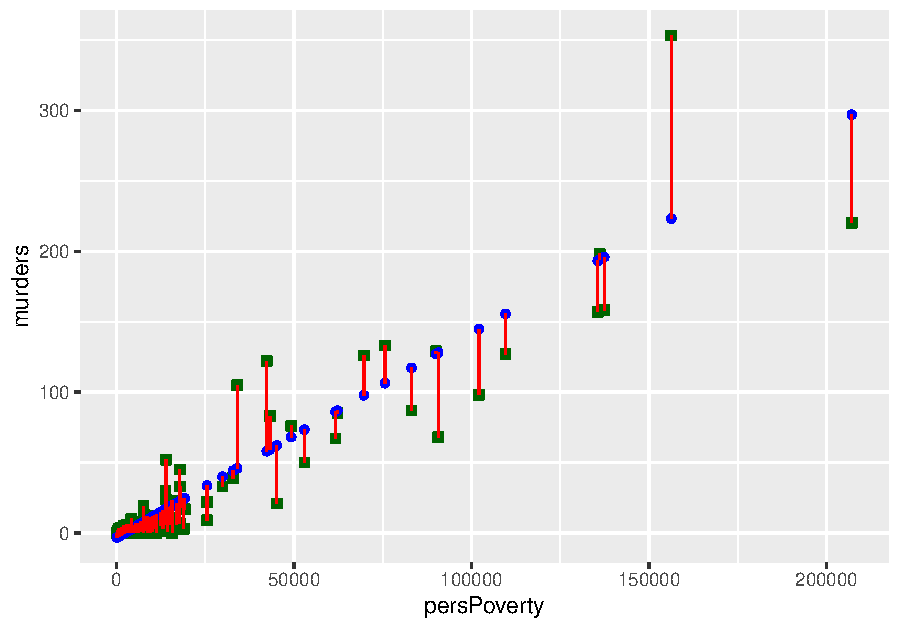
\includegraphics{_main_files/figure-latex/unnamed-chunk-13-1} 

}

\caption{Les segments en rouges représentent les résidus, les carrés verts les y non entrainés qui ont servi au test et les points bleus représentent les y prédits à partir de notre modèle.}\label{fig:unnamed-chunk-13}
\end{figure}

On peut aussi visualiser la répartition des résidus du modèle \texttt{lmSimple} autour de leur moyenne \(0\).\\

\begin{Shaded}
\begin{Highlighting}[]
\FunctionTok{plot}\NormalTok{(lmSimple}\SpecialCharTok{$}\NormalTok{residuals)}
\end{Highlighting}
\end{Shaded}

\begin{figure}

{\centering 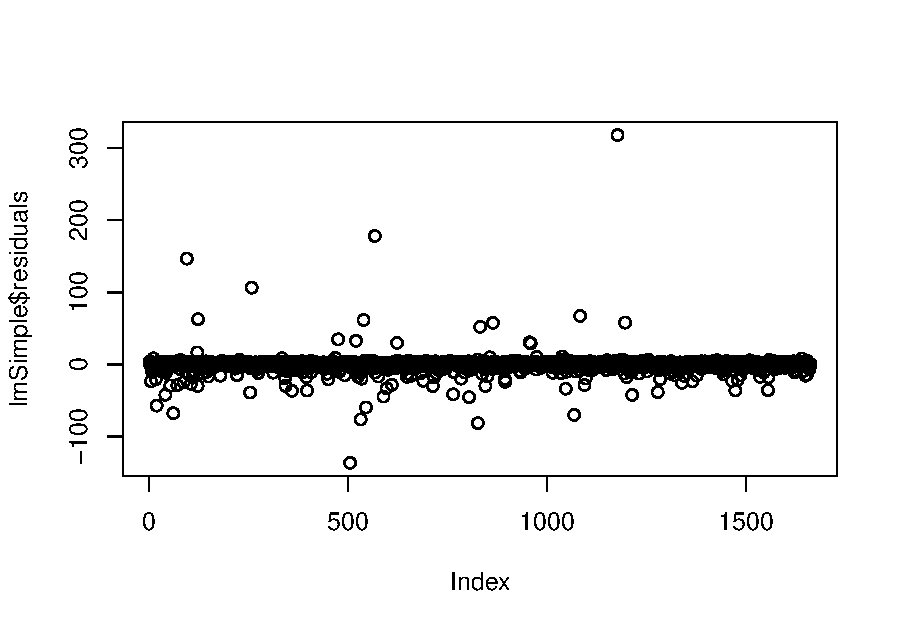
\includegraphics{_main_files/figure-latex/unnamed-chunk-14-1} 

}

\caption{On constate une répartition des résidus autour de 0}\label{fig:unnamed-chunk-14}
\end{figure}

\hypertarget{application-de-la-ruxe9gression-linuxe9aire-multiple}{%
\section{Application de la régression linéaire multiple}\label{application-de-la-ruxe9gression-linuxe9aire-multiple}}

Dans cette partie on peut s'intéresser à la relation entre le nombre de meurtres et plusieurs autres variables. Un modèle de régression linéaire multiple pourrait faire l'affaire. Comme dans le cas de la régression linéaire simple, on va commencer par étudier la corrélation entre les variables explicatives. Nous allons choisir dans notre exemple, les variables qui sont corrélées avec \texttt{murders} comme varioles indépendantes.\\
Ces dernières ne doivent pas être parfaitement corrélées entre elles. En effet dans la solution estimée du coefficient \(\beta\), on devra inversé la matrice X des variables explicatives. De ce fait une corrélation impliquera que la matrice ne soit pas de rang plein, donc non inversible.
\[\hat\beta = (X'X)^{-1}(X'y)\]
Commençons par selectionner nos variables pour la régression linéaire multiple.

\begin{Shaded}
\begin{Highlighting}[]
\FunctionTok{library}\NormalTok{(dplyr)}
\NormalTok{lmMultpleDF }\OtherTok{=}\NormalTok{ Communities }\SpecialCharTok{\%\textgreater{}\%} \FunctionTok{select}\NormalTok{(murders,pop, persUrban, persPoverty,}
\NormalTok{                           kidsBornNevrMarr, numForeignBorn,}
\NormalTok{                           houseVacant, persEmergShelt, persHomeless)}
\end{Highlighting}
\end{Shaded}

\hypertarget{entrauxeenement-de-moduxe8le}{%
\subsection*{Entraînement de modèle}\label{entrauxeenement-de-moduxe8le}}
\addcontentsline{toc}{subsection}{Entraînement de modèle}

Le langage R permet d'entraîner le modèle linéaire multiple grâce à la fonction \texttt{lm()}. Pour indiquer à la fonction que nous sommes dans le cas d'une régression multiple, l'argument \texttt{formula()} doit recevoir \texttt{y\textasciitilde{}X1+X2+...+XP} et pour notre exemple \texttt{murders\textasciitilde{}pop+persUrban+...}.
Lors qu'on précise l'argument data de la fonction lm et que les données ne contiennent que les variables à étudier, l'argument formula peut dans ce cas recevoir juste \texttt{y\textasciitilde{}.}. En Pratique, pour notre jeu de données \texttt{lmMultpleDF}, voici le code approprié :

\begin{Shaded}
\begin{Highlighting}[]
\CommentTok{\# train test split}
\NormalTok{lmMultiple\_Test }\OtherTok{=}\NormalTok{ lmMultpleDF[echantillon,]}
\NormalTok{lmMultiple\_Train }\OtherTok{=}\NormalTok{ lmMultpleDF[}\SpecialCharTok{{-}}\NormalTok{echantillon,]}
\CommentTok{\# Model training}
\NormalTok{lmMultiple }\OtherTok{=} \FunctionTok{lm}\NormalTok{(}\AttributeTok{formula =}\NormalTok{  murders}\SpecialCharTok{\textasciitilde{}}\NormalTok{.,}\AttributeTok{data =}\NormalTok{ lmMultiple\_Train)}
\FunctionTok{summary}\NormalTok{(lmMultiple)}
\end{Highlighting}
\end{Shaded}

\begin{verbatim}
## 
## Call:
## lm(formula = murders ~ ., data = lmMultiple_Train)
## 
## Residuals:
##      Min       1Q   Median       3Q      Max 
## -109.924   -1.099    0.412    1.206  175.748 
## 
## Coefficients:
##                    Estimate Std. Error t value Pr(>|t|)    
## (Intercept)      -4.318e-01  3.698e-01  -1.168 0.243166    
## pop              -1.096e-04  3.312e-05  -3.310 0.000953 ***
## persUrban         1.071e-05  2.910e-05   0.368 0.713030    
## persPoverty       2.131e-04  6.680e-05   3.190 0.001452 ** 
## kidsBornNevrMarr  3.119e-03  1.196e-04  26.080  < 2e-16 ***
## numForeignBorn    3.743e-04  1.809e-05  20.695  < 2e-16 ***
## houseVacant       1.824e-03  1.338e-04  13.629  < 2e-16 ***
## persEmergShelt    6.397e-03  1.853e-03   3.452 0.000571 ***
## persHomeless     -4.637e-02  4.110e-03 -11.282  < 2e-16 ***
## ---
## Signif. codes:  0 '***' 0.001 '**' 0.01 '*' 0.05 '.' 0.1 ' ' 1
## 
## Residual standard error: 10.41 on 1653 degrees of freedom
## Multiple R-squared:  0.9747, Adjusted R-squared:  0.9746 
## F-statistic:  7972 on 8 and 1653 DF,  p-value: < 2.2e-16
\end{verbatim}

La sortie de la fonction \texttt{summary()} indique qu'on peut se passer de la variable \texttt{persUrban} dans l'explication de \texttt{murders} par un modèle linéaire. En effet, son coefficient \(\beta\) pourrait être nul car les \(p-values\) est supérieure à \(\alpha=5\%\).\\

\begin{Shaded}
\begin{Highlighting}[]
\FunctionTok{library}\NormalTok{(dplyr)}
\DocumentationTok{\#\# Train test split}
\NormalTok{lmMultpleDF }\OtherTok{=}\NormalTok{ lmMultpleDF }\SpecialCharTok{\%\textgreater{}\%} \FunctionTok{select}\NormalTok{(}\SpecialCharTok{{-}}\NormalTok{persUrban)}
\NormalTok{lmMultiple\_Test }\OtherTok{=}\NormalTok{ lmMultpleDF[echantillon,]}
\NormalTok{lmMultiple\_Train }\OtherTok{=}\NormalTok{ lmMultpleDF[}\SpecialCharTok{{-}}\NormalTok{echantillon,]}
\CommentTok{\# Model training}
\NormalTok{lmMultiple }\OtherTok{=} \FunctionTok{lm}\NormalTok{(}\AttributeTok{formula =}\NormalTok{  murders}\SpecialCharTok{\textasciitilde{}}\NormalTok{.,}\AttributeTok{data =}\NormalTok{ lmMultiple\_Train)}
\FunctionTok{summary}\NormalTok{(lmMultiple)}
\end{Highlighting}
\end{Shaded}

\begin{verbatim}
## 
## Call:
## lm(formula = murders ~ ., data = lmMultiple_Train)
## 
## Residuals:
##      Min       1Q   Median       3Q      Max 
## -110.080   -1.137    0.422    1.222  175.907 
## 
## Coefficients:
##                    Estimate Std. Error t value Pr(>|t|)    
## (Intercept)      -5.027e-01  3.155e-01  -1.593 0.111255    
## pop              -9.813e-05  1.092e-05  -8.983  < 2e-16 ***
## persPoverty       2.098e-04  6.619e-05   3.170 0.001555 ** 
## kidsBornNevrMarr  3.122e-03  1.194e-04  26.150  < 2e-16 ***
## numForeignBorn    3.739e-04  1.804e-05  20.720  < 2e-16 ***
## houseVacant       1.822e-03  1.337e-04  13.630  < 2e-16 ***
## persEmergShelt    6.371e-03  1.851e-03   3.441 0.000593 ***
## persHomeless     -4.644e-02  4.105e-03 -11.312  < 2e-16 ***
## ---
## Signif. codes:  0 '***' 0.001 '**' 0.01 '*' 0.05 '.' 0.1 ' ' 1
## 
## Residual standard error: 10.41 on 1654 degrees of freedom
## Multiple R-squared:  0.9747, Adjusted R-squared:  0.9746 
## F-statistic:  9116 on 7 and 1654 DF,  p-value: < 2.2e-16
\end{verbatim}

De plus, le coefficient d'ajustement \(R^2\) est de \(0.9747\), soit un score de \(97.47\%\) pour notre modèle ce qui est un très bon résultat.

\hypertarget{graphes-de-ruxe9gression}{%
\subsection*{Graphes de régression}\label{graphes-de-ruxe9gression}}
\addcontentsline{toc}{subsection}{Graphes de régression}

Lorsque le nombre de variables explicatives dépasse \(2\), il est impossible de représenter sur un même graphes le nuage de points formé par y. En effet la dimension physique maximale est de 3.
Il existe plusieurs packages qui donnent des représentations assez significatives en deux dimensions du modèle linéaire multiple tel que \texttt{car}\footnote{package car : \url{https://cran.r-project.org/web/packages/car/index.html}}.\\
La représentation de la droite de régression peut se faire sur chaque dimension des variables explicatives grâce à la fonction \texttt{avPlots()} de la librairie \texttt{car}.

\begin{Shaded}
\begin{Highlighting}[]
\FunctionTok{library}\NormalTok{(car)}
\FunctionTok{avPlots}\NormalTok{(lmMultiple)}
\end{Highlighting}
\end{Shaded}

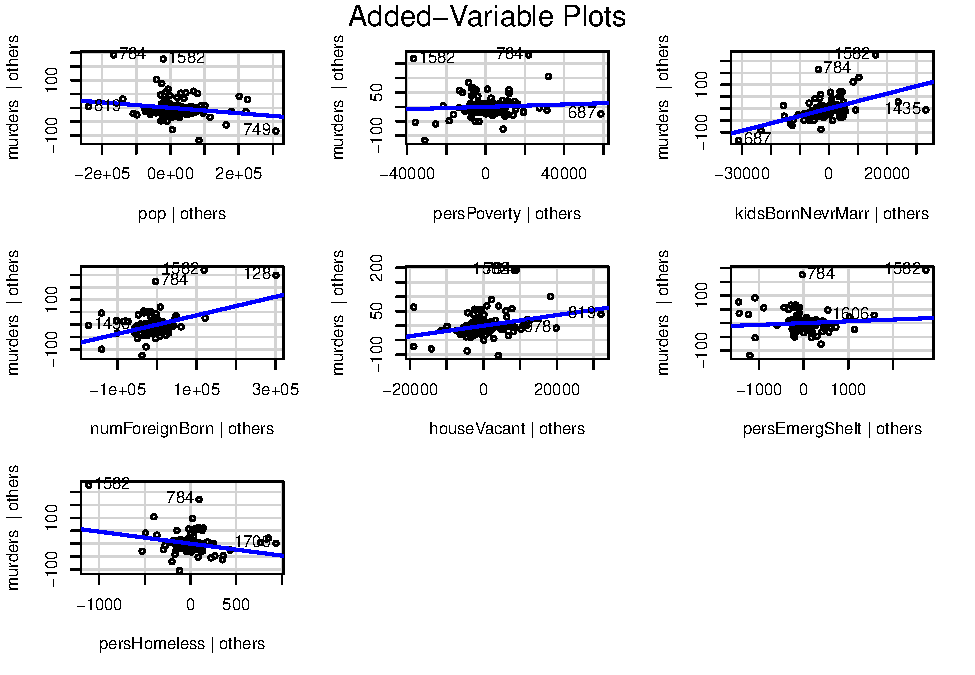
\includegraphics{_main_files/figure-latex/unnamed-chunk-18-1.pdf}

\hypertarget{pruxe9diction-1}{%
\subsection*{Prédiction}\label{pruxe9diction-1}}
\addcontentsline{toc}{subsection}{Prédiction}

La prédiction dans le modèle linéaire multiple se fait aussi avec la fonction \texttt{predict()} comme dans le cas simple. On va utiliser notre modèle déjà entraîné avec \(75\%\) de notre jeu de données \texttt{lmMultpleDF} et les \(20\%\) pour effectuer une prédiction. Cela peut nous permettre de voir les résidus entre les valeurs prédites et les valeurs réelles de \(y\).

\begin{Shaded}
\begin{Highlighting}[]
\NormalTok{y\_hat }\OtherTok{=} \FunctionTok{predict}\NormalTok{(lmMultiple,lmMultiple\_Test[,}\SpecialCharTok{{-}}\DecValTok{1}\NormalTok{])}
\FunctionTok{head}\NormalTok{(y\_hat,}\DecValTok{10}\NormalTok{)}
\end{Highlighting}
\end{Shaded}

\begin{verbatim}
##       2037        174        210        683        821        519       1593 
##  0.2445685 19.3517750  1.4280286  5.4097354  7.8093372  0.8155394 -1.6654378 
##       1098       1266       1153 
##  1.5812592 -1.1213912 -0.7649363
\end{verbatim}

\hypertarget{graphe-des-ruxe9sidus}{%
\subsection{Graphe des résidus}\label{graphe-des-ruxe9sidus}}

On peut visualiser les résidus entre les variables \(y_i\) observés et les \(\hat y_i\) prédites :

\begin{Shaded}
\begin{Highlighting}[]
\NormalTok{y\_test }\OtherTok{=}\NormalTok{ lmMultiple\_Test}\SpecialCharTok{$}\NormalTok{murders}
\FunctionTok{ggplot}\NormalTok{() }\SpecialCharTok{+}
  \FunctionTok{geom\_point}\NormalTok{(}\FunctionTok{aes}\NormalTok{(}\AttributeTok{x =}\NormalTok{ y\_test, }\AttributeTok{y =}\NormalTok{ y\_hat)) }\SpecialCharTok{+}
  \FunctionTok{geom\_abline}\NormalTok{(}\AttributeTok{slope =} \DecValTok{1}\NormalTok{, }\AttributeTok{color =}\StringTok{\textquotesingle{}blue\textquotesingle{}}\NormalTok{) }\SpecialCharTok{+}
  \FunctionTok{geom\_segment}\NormalTok{(}\FunctionTok{aes}\NormalTok{(}\AttributeTok{x =}\NormalTok{y\_test , }
                   \AttributeTok{y =}\NormalTok{ y\_test, }\AttributeTok{xend =}\NormalTok{ y\_test, }\AttributeTok{yend =}\NormalTok{ y\_hat),}
               \AttributeTok{color =} \StringTok{\textquotesingle{}red\textquotesingle{}}\NormalTok{) }\SpecialCharTok{+}
  \FunctionTok{ylab}\NormalTok{(}\StringTok{"Predicted murders"}\NormalTok{)}\SpecialCharTok{+}\FunctionTok{xlab}\NormalTok{(}\StringTok{"Murders"}\NormalTok{)}
\end{Highlighting}
\end{Shaded}

\begin{figure}
\centering
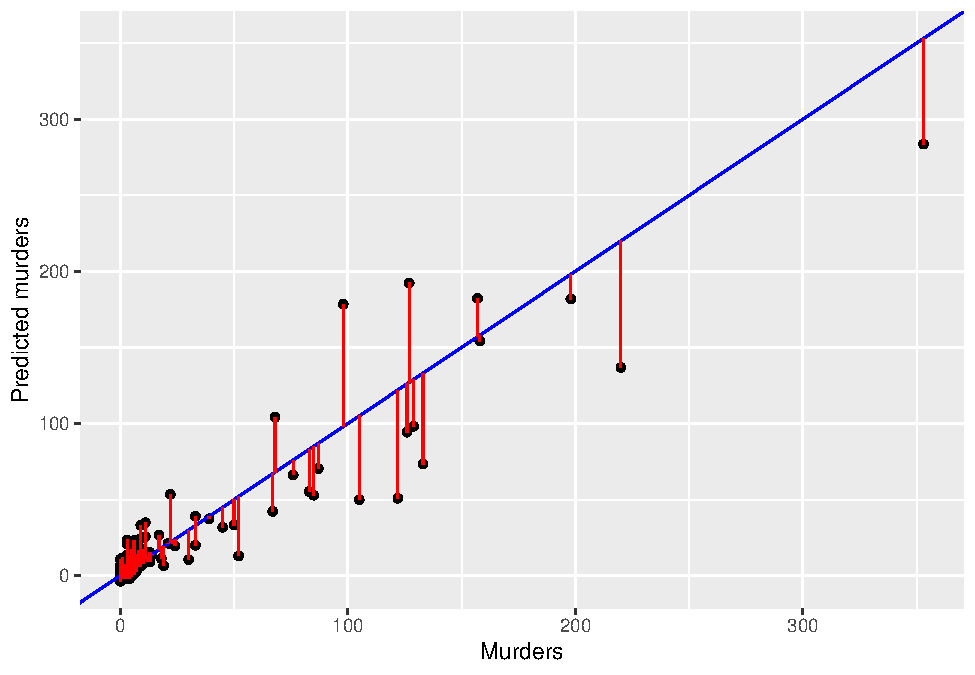
\includegraphics{_main_files/figure-latex/unnamed-chunk-20-1.pdf}
\caption{\label{fig:unnamed-chunk-20}Les résidus sont assez proches de 0 cela reflète la bonne qualité du modèle.}
\end{figure}

\hypertarget{principal-component-analysis-and-factor-analysis}{%
\chapter{Principal Component Analysis and Factor Analysis}\label{principal-component-analysis-and-factor-analysis}}

Nous allons effectuer une Analyse en Composantes Principales(ACP) pour la variables numériques de notre jeu de données \texttt{Communities}

\hypertarget{suxe9lection-des-variables-numuxe9riques}{%
\subsection*{Sélection des variables numériques}\label{suxe9lection-des-variables-numuxe9riques}}
\addcontentsline{toc}{subsection}{Sélection des variables numériques}

\begin{Shaded}
\begin{Highlighting}[]
\FunctionTok{library}\NormalTok{(dplyr)}
\NormalTok{PCA\_df }\OtherTok{\textless{}{-}}\NormalTok{ Communities }\SpecialCharTok{\%\textgreater{}\%} \FunctionTok{select\_if}\NormalTok{(is.numeric)}
\end{Highlighting}
\end{Shaded}

\hypertarget{application-de-la-fonction-pca}{%
\subsection*{Application de la fonction PCA}\label{application-de-la-fonction-pca}}
\addcontentsline{toc}{subsection}{Application de la fonction PCA}

L'objectif est de réduire la dimension de notre jeu de données \texttt{PCA\_df} tout en conservant un pourcentage élevé des informations.

\begin{Shaded}
\begin{Highlighting}[]
\NormalTok{Communities\_PCA }\OtherTok{\textless{}{-}}\NormalTok{ FactoMineR}\SpecialCharTok{::}\FunctionTok{PCA}\NormalTok{(PCA\_df,}\AttributeTok{scale.unit=}\ConstantTok{TRUE}\NormalTok{,}
                                   \AttributeTok{graph =} \ConstantTok{FALSE}\NormalTok{)}
\end{Highlighting}
\end{Shaded}

\hypertarget{pourcentage-dexplication}{%
\subsection*{Pourcentage d'explication}\label{pourcentage-dexplication}}
\addcontentsline{toc}{subsection}{Pourcentage d'explication}

\begin{Shaded}
\begin{Highlighting}[]
\NormalTok{factoextra}\SpecialCharTok{::}\FunctionTok{fviz\_eig}\NormalTok{(Communities\_PCA,}\AttributeTok{addlabels =} \ConstantTok{TRUE}\NormalTok{)}
\end{Highlighting}
\end{Shaded}

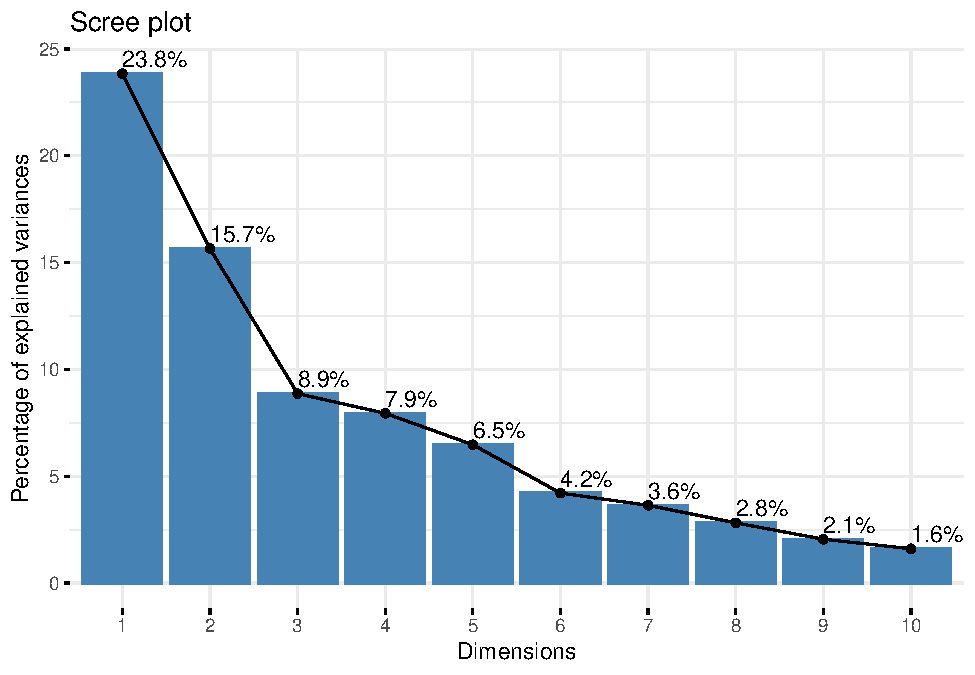
\includegraphics{_main_files/figure-latex/unnamed-chunk-24-1.pdf}

Nous constatons que deux dimensions sont insuffisantes pour représenter 75\% des informations. Pour y remédier nous allons diminuer le nombre de variables de \texttt{PCA\_df}(6 par exemple).

\begin{Shaded}
\begin{Highlighting}[]
\FunctionTok{library}\NormalTok{(dplyr)}
\NormalTok{PCA\_df }\OtherTok{=}\NormalTok{ PCA\_df }\SpecialCharTok{\%\textgreater{}\%} \FunctionTok{select}\NormalTok{(murders,pctWhite,pctBlack,}
\NormalTok{                           pctKidsBornNevrMarr,}
\NormalTok{                           numForeignBorn,pctUnemploy)}
\NormalTok{Communities\_PCA }\OtherTok{\textless{}{-}}\NormalTok{ FactoMineR}\SpecialCharTok{::}\FunctionTok{PCA}\NormalTok{(PCA\_df,}\AttributeTok{scale.unit=}\ConstantTok{TRUE}\NormalTok{,}
                                   \AttributeTok{graph =}\NormalTok{ F)}
\NormalTok{factoextra}\SpecialCharTok{::}\FunctionTok{fviz\_eig}\NormalTok{(Communities\_PCA,}\AttributeTok{addlabels =} \ConstantTok{TRUE}\NormalTok{)}
\end{Highlighting}
\end{Shaded}

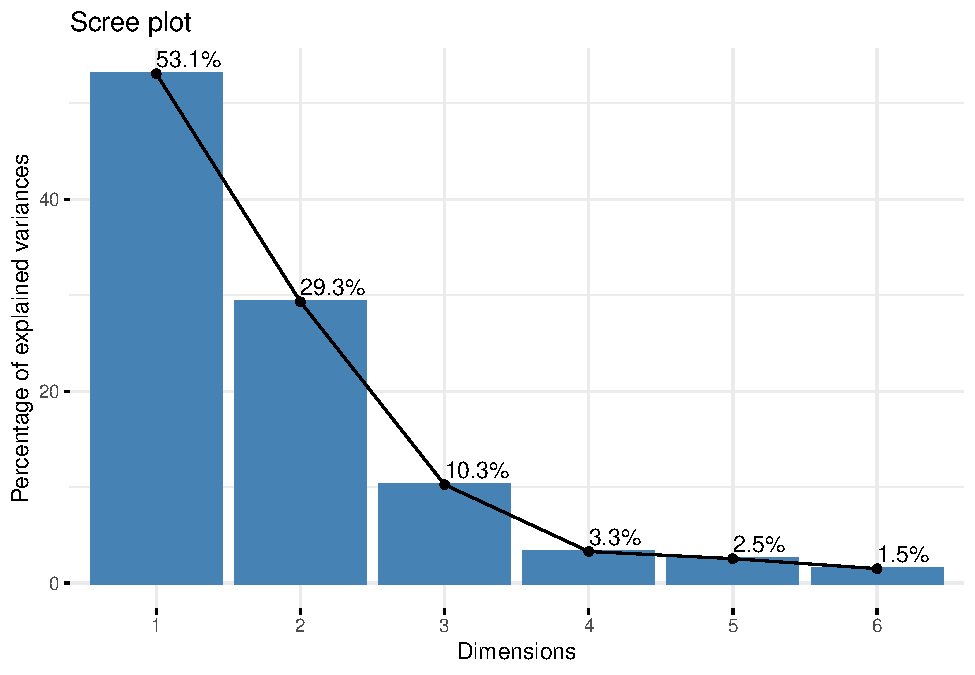
\includegraphics{_main_files/figure-latex/unnamed-chunk-25-1.pdf}
Ce graphe nous permet de remarquer que deux composantes principales sont suiffisantes pour représenter \(82.4\%\) de l'information ce qui est supérieur à \(75\%\) notre pourcentage seuil.\\

\hypertarget{graphiques-de-corruxe9lation-des-variables}{%
\subsection*{Graphiques de corrélation des variables}\label{graphiques-de-corruxe9lation-des-variables}}
\addcontentsline{toc}{subsection}{Graphiques de corrélation des variables}

\begin{Shaded}
\begin{Highlighting}[]
\NormalTok{factoextra}\SpecialCharTok{::}\FunctionTok{fviz\_pca\_var}\NormalTok{(Communities\_PCA,}
             \AttributeTok{col.var =} \StringTok{"contrib"}\NormalTok{, }
             \AttributeTok{gradient.cols =} \FunctionTok{rainbow}\NormalTok{(}\DecValTok{3}\NormalTok{),}
             \AttributeTok{repel =} \ConstantTok{TRUE}\NormalTok{,}
             \AttributeTok{legend.title=}\StringTok{\textquotesingle{}Contribution\textquotesingle{}}\NormalTok{)}
\end{Highlighting}
\end{Shaded}

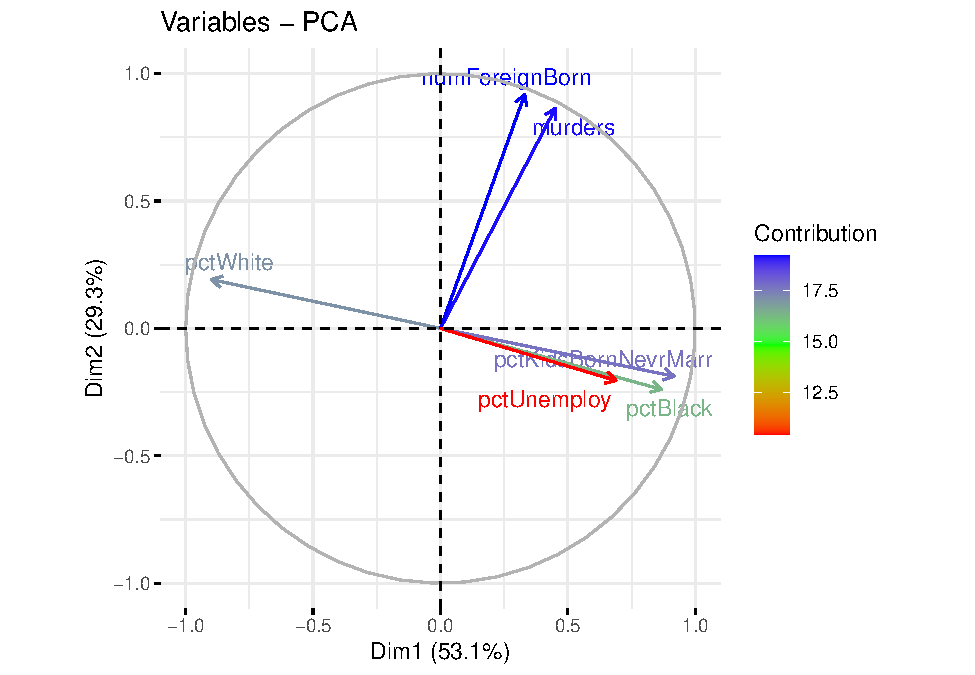
\includegraphics{_main_files/figure-latex/unnamed-chunk-26-1.pdf}

À partie du graphe précédent, nous pouvons constater une forte corrélation entre le pourcentage de personnes sans emplois \texttt{pctUnemploy}, d'enfants nés hors mariage \texttt{pctKidsBornNevrMarr} et de personnes de la communauté noire américaine \texttt{pctBlack}. Ces dernières sont peu corrélées avec \texttt{murders}.

\hypertarget{graphes-des-individus}{%
\subsection*{Graphes des individus}\label{graphes-des-individus}}
\addcontentsline{toc}{subsection}{Graphes des individus}

\begin{Shaded}
\begin{Highlighting}[]
\NormalTok{factoextra}\SpecialCharTok{::}\FunctionTok{fviz\_pca\_ind}\NormalTok{(Communities\_PCA,}
                 \AttributeTok{col.ind =}\StringTok{\textquotesingle{}cos2\textquotesingle{}}\NormalTok{,}
                 \AttributeTok{gradient.cols =} \FunctionTok{rainbow}\NormalTok{(}\DecValTok{10}\NormalTok{),}
                 \AttributeTok{repel =} \ConstantTok{TRUE}\NormalTok{,}
                 \AttributeTok{legend.title =} \StringTok{"Cos2 for the variables"}\NormalTok{,}
\NormalTok{                 )}
\end{Highlighting}
\end{Shaded}

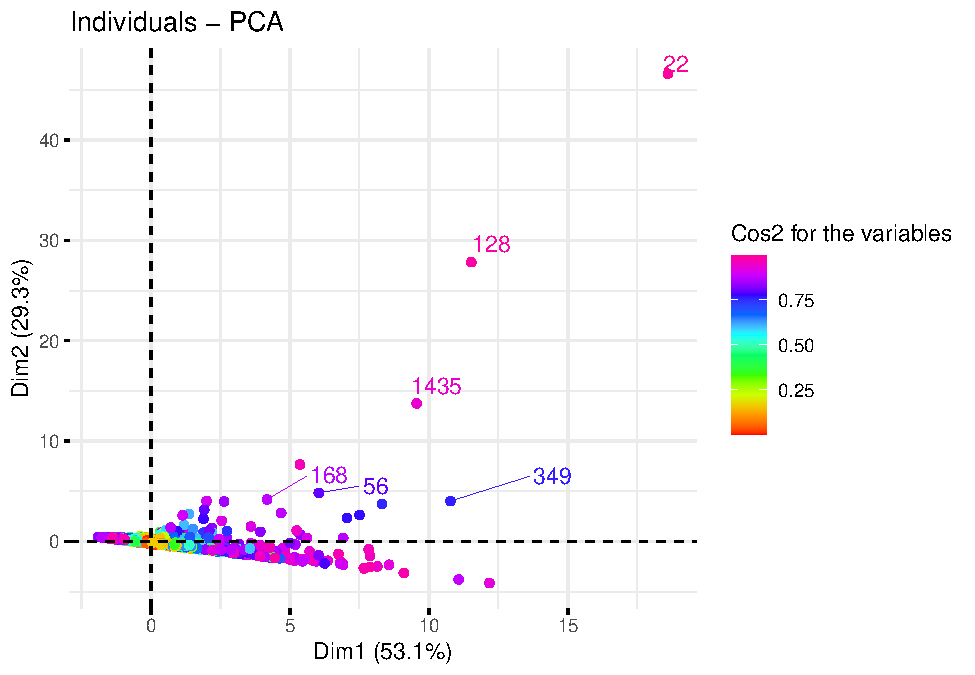
\includegraphics{_main_files/figure-latex/unnamed-chunk-27-1.pdf}

Une variable avec un score élevé suivant un axe signifie qu'elle a fortement contribué à la création de cet axe. Une variable moyenne c'est celle qui est proche de l'origine.

\hypertarget{biplot-individus-et-variables}{%
\subsection*{Biplot individus et variables}\label{biplot-individus-et-variables}}
\addcontentsline{toc}{subsection}{Biplot individus et variables}

\begin{Shaded}
\begin{Highlighting}[]
\NormalTok{factoextra}\SpecialCharTok{::}\FunctionTok{fviz\_pca\_biplot}\NormalTok{(Communities\_PCA, }\AttributeTok{repel =} \ConstantTok{TRUE}\NormalTok{,}
                \AttributeTok{col.var =} \FunctionTok{rainbow}\NormalTok{(}\DecValTok{4}\NormalTok{)[}\DecValTok{4}\NormalTok{], }
                \AttributeTok{col.ind =} \FunctionTok{rainbow}\NormalTok{(}\DecValTok{1}\NormalTok{)}
\NormalTok{                )}
\end{Highlighting}
\end{Shaded}

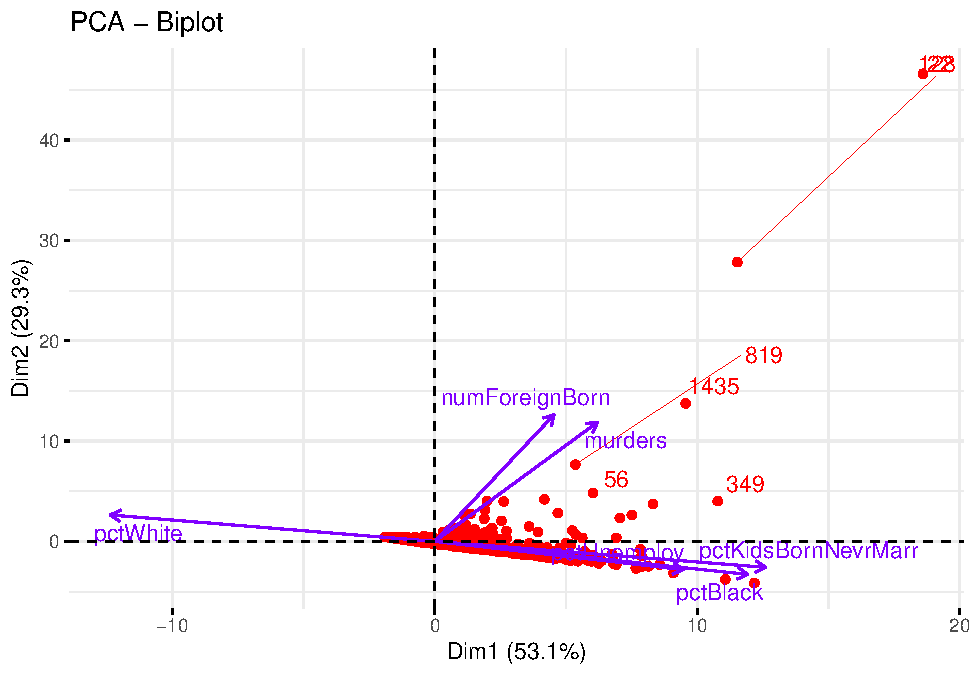
\includegraphics{_main_files/figure-latex/unnamed-chunk-28-1.pdf}

Prenons la la variable numéro 819 (C'est à dire la ligne 819 de \texttt{PCA\_df}). Nous savons que les variables \{murders\} et \{numForeignBorn\} sont fortement corrélées. Alors si le nombre de meutres \{murders\} est très faible par rapport à la moyenne, alors le nombre de personnes nées à l'étranger\{numForeignBorn\} l'est aussi.\\

Un raisonnement similaire peut être fait pour les variable fortement et négativement corrélées comme le pourcentage de personnes sans emplois \texttt{pctUnemploy} et de personnes de la communauté blanche américaine \texttt{pctWhite} sauf que dans ce cas, les variables varieront dans de sens opposés.
Nous pouvons vérifier ces informations tirées sur le graphes précédent dans notre data set grâce à la cellule de code suivante.

\begin{Shaded}
\begin{Highlighting}[]
\FunctionTok{library}\NormalTok{(dplyr)}
\NormalTok{variable819 }\OtherTok{\textless{}{-}} \FunctionTok{rbind}\NormalTok{(PCA\_df[}\DecValTok{819}\NormalTok{,],}\FunctionTok{apply}\NormalTok{(PCA\_df,}\DecValTok{2}\NormalTok{,mean),}
                   \FunctionTok{apply}\NormalTok{(PCA\_df,}\DecValTok{2}\NormalTok{,min),}
                   \FunctionTok{apply}\NormalTok{(PCA\_df,}\DecValTok{2}\NormalTok{,max)}
\NormalTok{                   ) }\SpecialCharTok{\%\textgreater{}\%}\NormalTok{  dplyr}\SpecialCharTok{::}\FunctionTok{select}\NormalTok{(murders,numForeignBorn) }\SpecialCharTok{\%\textgreater{}\%} 
                     \StringTok{\textasciigrave{}}\AttributeTok{rownames\textless{}{-}}\StringTok{\textasciigrave{}}\NormalTok{(.,}\FunctionTok{c}\NormalTok{(}\StringTok{\textquotesingle{}Variable819\textquotesingle{}}\NormalTok{,}\StringTok{\textquotesingle{}mean\textquotesingle{}}\NormalTok{,}\StringTok{\textquotesingle{}min\textquotesingle{}}\NormalTok{,}\StringTok{\textquotesingle{}max\textquotesingle{}}\NormalTok{))}
\NormalTok{variable819}
\end{Highlighting}
\end{Shaded}

\begin{verbatim}
##                 murders numForeignBorn
## Variable819  446.000000     290374.000
## mean           7.764786       6277.274
## min            0.000000         20.000
## max         1946.000000    2082931.000
\end{verbatim}

\hypertarget{lanalyse-de-la-variance}{%
\chapter{L'analyse de la variance}\label{lanalyse-de-la-variance}}

Dans cette section on va s'intéresser aux meurtres commis par unité de gang déployé \texttt{gangUnit}. Pour cette dernière, l'encodage est le suivant : 0 signifie ``Meaning'', 10 signifie ``Oui'' et 5 signifie temps partiel(``Part-Time'').\\

\hypertarget{suxe9lection-des-donnuxe9es}{%
\subsection*{Sélection des données}\label{suxe9lection-des-donnuxe9es}}
\addcontentsline{toc}{subsection}{Sélection des données}

On va sélectionner les données qui serviront l'ANOVA puis ajjouter une nouvelle collonne pour le décodage de \texttt{gangUnit}.

\begin{Shaded}
\begin{Highlighting}[]
\FunctionTok{library}\NormalTok{(dplyr)}
\NormalTok{aov\_data }\OtherTok{=}\NormalTok{ Communities }\SpecialCharTok{\%\textgreater{}\%} \FunctionTok{select}\NormalTok{(murders,gangUnit) }\SpecialCharTok{\%\textgreater{}\%} 
          \FunctionTok{mutate}\NormalTok{(}\AttributeTok{GangUnit\_means =} \FunctionTok{case\_when}\NormalTok{(gangUnit}\SpecialCharTok{==}\StringTok{"0"}\SpecialCharTok{\textasciitilde{}}\StringTok{"Non"}\NormalTok{,}
\NormalTok{                                     gangUnit}\SpecialCharTok{==}\StringTok{"10"}\SpecialCharTok{\textasciitilde{}}\StringTok{"Oui"}\NormalTok{,}
\NormalTok{                                     gangUnit}\SpecialCharTok{==}\StringTok{"5"}\SpecialCharTok{\textasciitilde{}}\StringTok{"Part{-}Time"}\NormalTok{,}
\NormalTok{                                     gangUnit}\SpecialCharTok{==}\StringTok{"?"}\SpecialCharTok{\textasciitilde{}}\ConstantTok{NA\_character\_}\NormalTok{))}
\end{Highlighting}
\end{Shaded}

\hypertarget{les-boites-uxe0-moustaches}{%
\subsection*{Les boites à moustaches}\label{les-boites-uxe0-moustaches}}
\addcontentsline{toc}{subsection}{Les boites à moustaches}

Le premier travail à faire lors d'une ANOVA est la représentation des boites à moustaches. Nous allons utliser le packages \emph{ggstatsplot}\footnote{\url{https://indrajeetpatil.github.io/ggstatsplot/}} qui donne une sortie avec plusieurs informations.

\begin{Shaded}
\begin{Highlighting}[]
\FunctionTok{library}\NormalTok{(ggstatsplot)}
\end{Highlighting}
\end{Shaded}

\begin{verbatim}
## You can cite this package as:
##      Patil, I. (2021). Visualizations with statistical details: The 'ggstatsplot' approach.
##      Journal of Open Source Software, 6(61), 3167, doi:10.21105/joss.03167
\end{verbatim}

\begin{Shaded}
\begin{Highlighting}[]
\FunctionTok{ggbetweenstats}\NormalTok{(}
  \AttributeTok{data =}\NormalTok{ aov\_data,}
  \AttributeTok{x     =}\NormalTok{ GangUnit\_means,}
  \AttributeTok{y     =}\NormalTok{ murders,}
  \AttributeTok{title =} \StringTok{"Boites à moustaches des crimes"}
\NormalTok{)}
\end{Highlighting}
\end{Shaded}

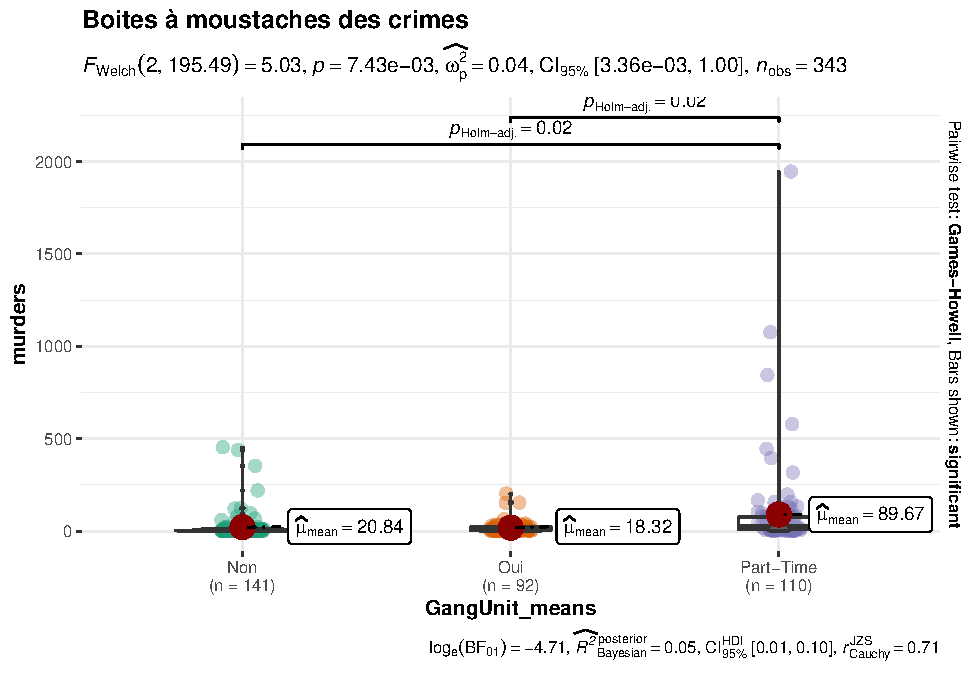
\includegraphics{_main_files/figure-latex/unnamed-chunk-32-1.pdf}

Dû à des valeurs manquantes, notre représentation porte sur \(343\) observations. Les boites à moustache indiquent qu'en moyenne, le nombre de meurtres varie lors que \texttt{gangUnit} change de modalité. Passons à l'anova pour en savoir plus.

\hypertarget{application-de-lanova-uxe0-un-facteur}{%
\subsection*{Application de l'anova à un facteur}\label{application-de-lanova-uxe0-un-facteur}}
\addcontentsline{toc}{subsection}{Application de l'anova à un facteur}

Le logiciel \textbf{R} nous permet de faire l'analyse de la variance grâce à la fonction \(aov()\).

\begin{Shaded}
\begin{Highlighting}[]
\NormalTok{murders\_aov }\OtherTok{=} \FunctionTok{aov}\NormalTok{(murders}\SpecialCharTok{\textasciitilde{}}\NormalTok{GangUnit\_means,}\AttributeTok{data =}\NormalTok{ aov\_data)}
\FunctionTok{summary}\NormalTok{(murders\_aov)}
\end{Highlighting}
\end{Shaded}

\begin{verbatim}
##                 Df  Sum Sq Mean Sq F value   Pr(>F)    
## GangUnit_means   2  364694  182347   9.377 0.000109 ***
## Residuals      340 6611431   19445                     
## ---
## Signif. codes:  0 '***' 0.001 '**' 0.01 '*' 0.05 '.' 0.1 ' ' 1
## 1872 observations deleted due to missingness
\end{verbatim}

Comme le laissaient paraître les boxplots, d'après le tableau précédent, la \(p-value=0.000109<\alpha=5\%\), alors l'effet de gang(\texttt{gangUnit}) sur le nombre de crimes est significatif.

  \bibliography{book.bib,packages.bib}

\end{document}
